\documentclass[a4paper,footinbib,final,openany,final,12pt]{book}

\usepackage[cyr]{aeguill}
\usepackage{xspace}
\usepackage[french]{babel}
%\usepackage{xunicode}
%\usepackage{ifxetex}
%\usepackage{fontspec}
\usepackage{slantsc}
%\usepackage{array}
\usepackage{amsmath}
%\pagestyle{empty}
%\usepackage[urw-garamond]{mathdesign}
\usepackage{rotating}
\usepackage{graphics}
\usepackage{graphicx}
\usepackage{color}
\usepackage{epsfig}
\usepackage{indentfirst}
%\usepackage[14pt]{moresize}
\usepackage[12pt]{moresize}
\usepackage[T1]{fontenc} % for French characters
%\usepackage[applemac]{inputenc}
\usepackage[utf8]{inputenc}
\usepackage{eurosym}
%\usepackage{fancy}
\usepackage{fancyhdr}
\usepackage{lettrine}
%\usepackage{times}

%\fontspec{Hoefler Text}
\setcounter{tocdepth}{4}

\author{\textsl{Jacques-B{\'{e}}nigne Bossuet}}
\title{\textsc{Sermon sur la mort}}

\oddsidemargin=0pt
\evensidemargin=0pt
\topmargin=-30pt
\headheight=15pt
\headsep=30pt
\textheight=670pt
\textwidth=470pt
\setlength{\parindent}{20pt}        % for indentation of 
\setlength{\parskip}{1.2ex}          % for spacing between paragraphs
\footskip=35pt
\voffset=0pt

\pagestyle{fancy}

\lhead{}
\chead{\textsc{\textsc{Sermon sur la mort}}}
\rhead{}

\begin{document}

\renewcommand{\thepart}{}
\renewcommand{\partname}{}
\renewcommand{\thechapter}{}
\renewcommand{\chaptername}{}
\renewcommand{\thesection}{}

\thispagestyle{empty}
\vspace*{18ex}
\begin{center}
\fontsize{100pt}{100pt}\selectfont
\textsc{Sermon sur la mort}\\
\vspace{3ex}
\fontsize{25pt}{25pt}\selectfont
\emph{{Jacques-B{\'{e}}nigne Bossuet}}
\end{center}
\newpage
\strut
\newpage

\vspace*{50ex}
\begin{flushright}
\emph{\textbf{\large{Intro\"{i}t}}}\\
\vspace*{2ex}
\large{\emph{{\normalsize{Il advint qu'un beau soir l'univers se brisa\\Sur des r{\'{e}}cifs que les naufrageurs enflamm{\`{e}}rent\\Moi je voyais briller au-dessus de la mer\\Les yeux d'Elsa les yeux d'Elsa les yeux d'Elsa }}}}
\end{flushright}
\newpage
\strut
\newpage
\tableofcontents
\newpage
\strut
\newpage

\section{Remerciements (ou pas)}

\lettrine{E}{n recevant} la distinction dont votre libre Acad{\'{e}}mie a bien voulu m'honorer, ma gratitude {\'{e}}tait d'autant plus profonde que je mesurais {\`{a}} quel point cette r{\'{e}}compense d{\'{e}}passait mes m{\'{e}}rites personnels. Tout homme et, {\`{a}} plus forte raison, tout artiste, d{\'{e}}sire {\^{e}}tre reconnu~\cite{Noyau}. Je le d{\'{e}}sire aussi. Mais il ne m'a pas {\'{e}}t{\'{e}} possible d'apprendre votre d{\'{e}}cision sans comparer son retentissement {\`{a}} ce que je suis r{\'{e}}ellement. Comment un homme presque jeune, riche de ses seuls doutes et d'une {\oe}uvre encore en chantier, habitu{\'{e}} {\`{a}} vivre dans la solitude du travail ou dans les retraites de l'amiti{\'{e}}, n'aurait-il pas appris avec une sorte de panique un arr{\^{e}}t qui le portait d'un coup, seul et r{\'{e}}duit {\`{a}} lui-m{\^{e}}me, au centre d'une lumi{\'{e}}re crue ? De quel c{\oe}ur aussi pouvait-il recevoir~\cite{Fondement} cet honneur {\`{a}} l'heure o{\`{u}}, en Europe, d'autres {\'{e}}crivains, parmi les plus grands, sont r{\'{e}}duits au silence, et dans le temps m{\^{e}}me o{\`{u}} sa terre natale conna{\^{i}}t un malheur incessant ?
\newpage
\strut
\newpage

\section{Introduction}
\begin{flushright}
\emph{\textbf{\small{Il y a diverses sortes de curiosit{\'{e}} : l'une d'int{\'{e}}r{\'{e}}t, qui nous porte {\`{a}} d{\'{e}}sirer d'apprendre ce qui nous peut {\'{e}}tre utile, et l'autre d'orgueil, qui vient du d{\'{e}}sir de savoir ce que les autres ignorent.}}}
\end{flushright}
Quoi que puisse dire Aristote et toute la Philosophie, il n'est rien d'{\'{e}}gal au tabac : c'est la passion des honn{\^{e}}tes gens, et qui vit sans tabac n'est pas digne de vivre~\cite{Revolution}. Non-seulement il r{\'{e}}jouit et purge les cerveaux humains, mais encore il instruit les {\`{a}}mes {\`{a}} la vertu, et l'on apprend avec lui {\`{a}} devenir honn{\^{e}}te homme. Ne voyez-vous pas bien, d{\`{e}}s qu'on en prend, de quelle mani{\`{e}}re obligeante on en use avec tout le monde, et comme on est ravi d'en donner {\`{a}} droit et {\`{a}} gauche, partout o{\`{u}} l'on se trouve ? On n'attend pas m{\^{e}}me qu'on en demande, et l'on court au-devant du souhait des gens : tant il est vrai que le tabac inspire des sentiments d'honneur et de vertu {\`{a}} tous ceux qui en prennent.
\newpage

\section{25 d{\'{e}}cembre 2017 : Complie}

Me sera-t-il permis aujourd'hui d'ouvrir un tombeau devant la cour, et des yeux si d{\'{e}}licats ne seront-ils point offens{\'{e}}s par un objet si fun{\`{e}}bre ? Je ne pense pas, messieurs, que des chr{\'{e}}tiens doivent refuser d'assister {\`{a}} ce spectacle avec J{\'{e}}sus-Christ \cite{Saminadayar}. C'est {\`{a}} lui que l'on dit dans notre {\'{e}}vangile : seigneur, venez, et voyez o{\`{u}} l'on a d{\'{e}}pos{\'{e}} le corps du Lazare ; c'est lui qui ordonne qu'on l{\`{e}}ve la pierre, et qui semble nous dire {\`{a}} son tour : venez, et voyez vous-m{\^{e}}mes~\cite{Parti}. J{\'{e}}sus ne refuse pas de voir ce corps mort, comme un objet de piti{\'{e}} et un sujet de miracle ; mais c'est nous, mortels mis{\'{e}}rables, qui refusons de voir ce triste spectacle, comme la conviction de nos erreurs. Allons, et voyons avec J{\'{e}}sus-Christ ; et d{\'{e}}sabusons-nous {\'{e}}ternellement de tous les biens que la mort enl{\`{e}}ve.

\begin{figure}[!htb]
\begin{center}
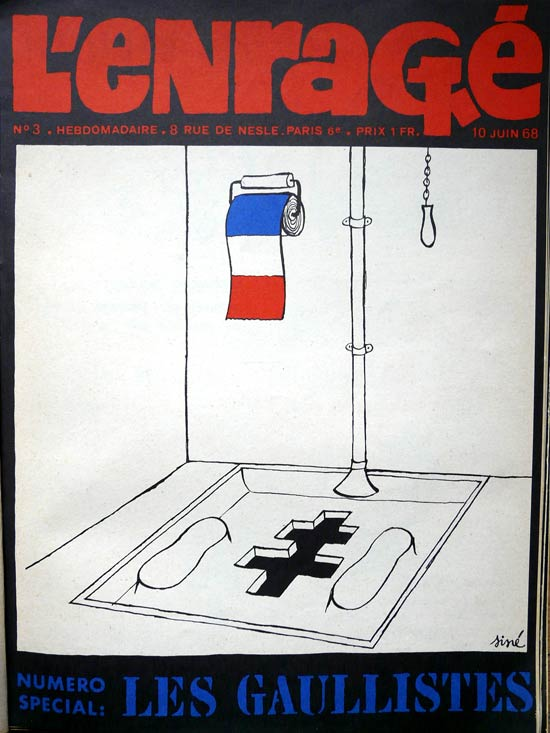
\includegraphics[width=8cm]{Fig01}
\caption{N'esp{\'{e}}rez pas trop de l'{\'{e}}tat. Il ne peut donner que ce qu'il re{\c{c}}oit.}
\label{Fig1}
\end{center}
\end{figure}

C'est une {\'{e}}trange faiblesse de l'esprit humain que jamais la mort ne lui soit pr{\'{e}}sente, quoiqu'elle se mette en vue de tous c{\^{o}}t{\'{e}}s, et en mille formes diverses. On n'entend dans les fun{\'{e}}railles que des paroles d'{\'{e}}tonnement de ce que ce mortel est mort. Chacun rappelle en son souvenir depuis quel temps il lui a parl{\'{e}}, et de quoi le d{\'{e}}funt l'a entretenu ; et tout d'un coup il est mort. Voil{\`{a}}, dit-on, ce que c'est que l'homme ! Et celui qui le dit, c'est un homme ; et cet homme ne s'applique rien, oublieux de sa destin{\'{e}}e ! Ou s'il passe dans son esprit quelque d{\'{e}}sir volage de s'y pr{\'{e}}parer, il dissipe bient{\^{o}}t ces noires id{\'{e}}es ; et je puis dire, messieurs, que les mortels n'ont pas moins de soin d'ensevelir les pens{\'{e}}es de la mort que d'enterrer les morts m{\^{e}}mes. Mais peut-{\^{e}}tre que ces pens{\'{e}}es feront plus d'effet dans nos coeurs, si nous les m{\'{e}}ditons avec J{\'{e}}sus-Christ sur le tombeau du Lazare ; mais demandons-lui qu'il nous les imprime par la gr{\`{a}}ce de son saint-esprit, et t{\^{a}}chons de la m{\'{e}}riter par l'entremise de la sainte Vierge~\cite{Efforts,Communiste}.
				
\section{Jour de l'An 2017 : Matines}

 {\c{C}}a a d{\'{e}}but{\'{e}} comme {\c{c}}a. Moi, j'avais jamais rien dit. Rien. C'est Arthur Ganate qui m'a fait parler. Arthur, un {\'{e}}tudiant, un carabin lui aussi, un camarade. On se rencontre donc place Clichy. C'{\'{e}}tait apr{\`{e}}s le d{\'{e}}jeuner. Il veut me parler. Je l'{\'{e}}coute. \og Restons pas dehors ! qu'il me dit.

\begin{figure}[!htb]
\begin{center}
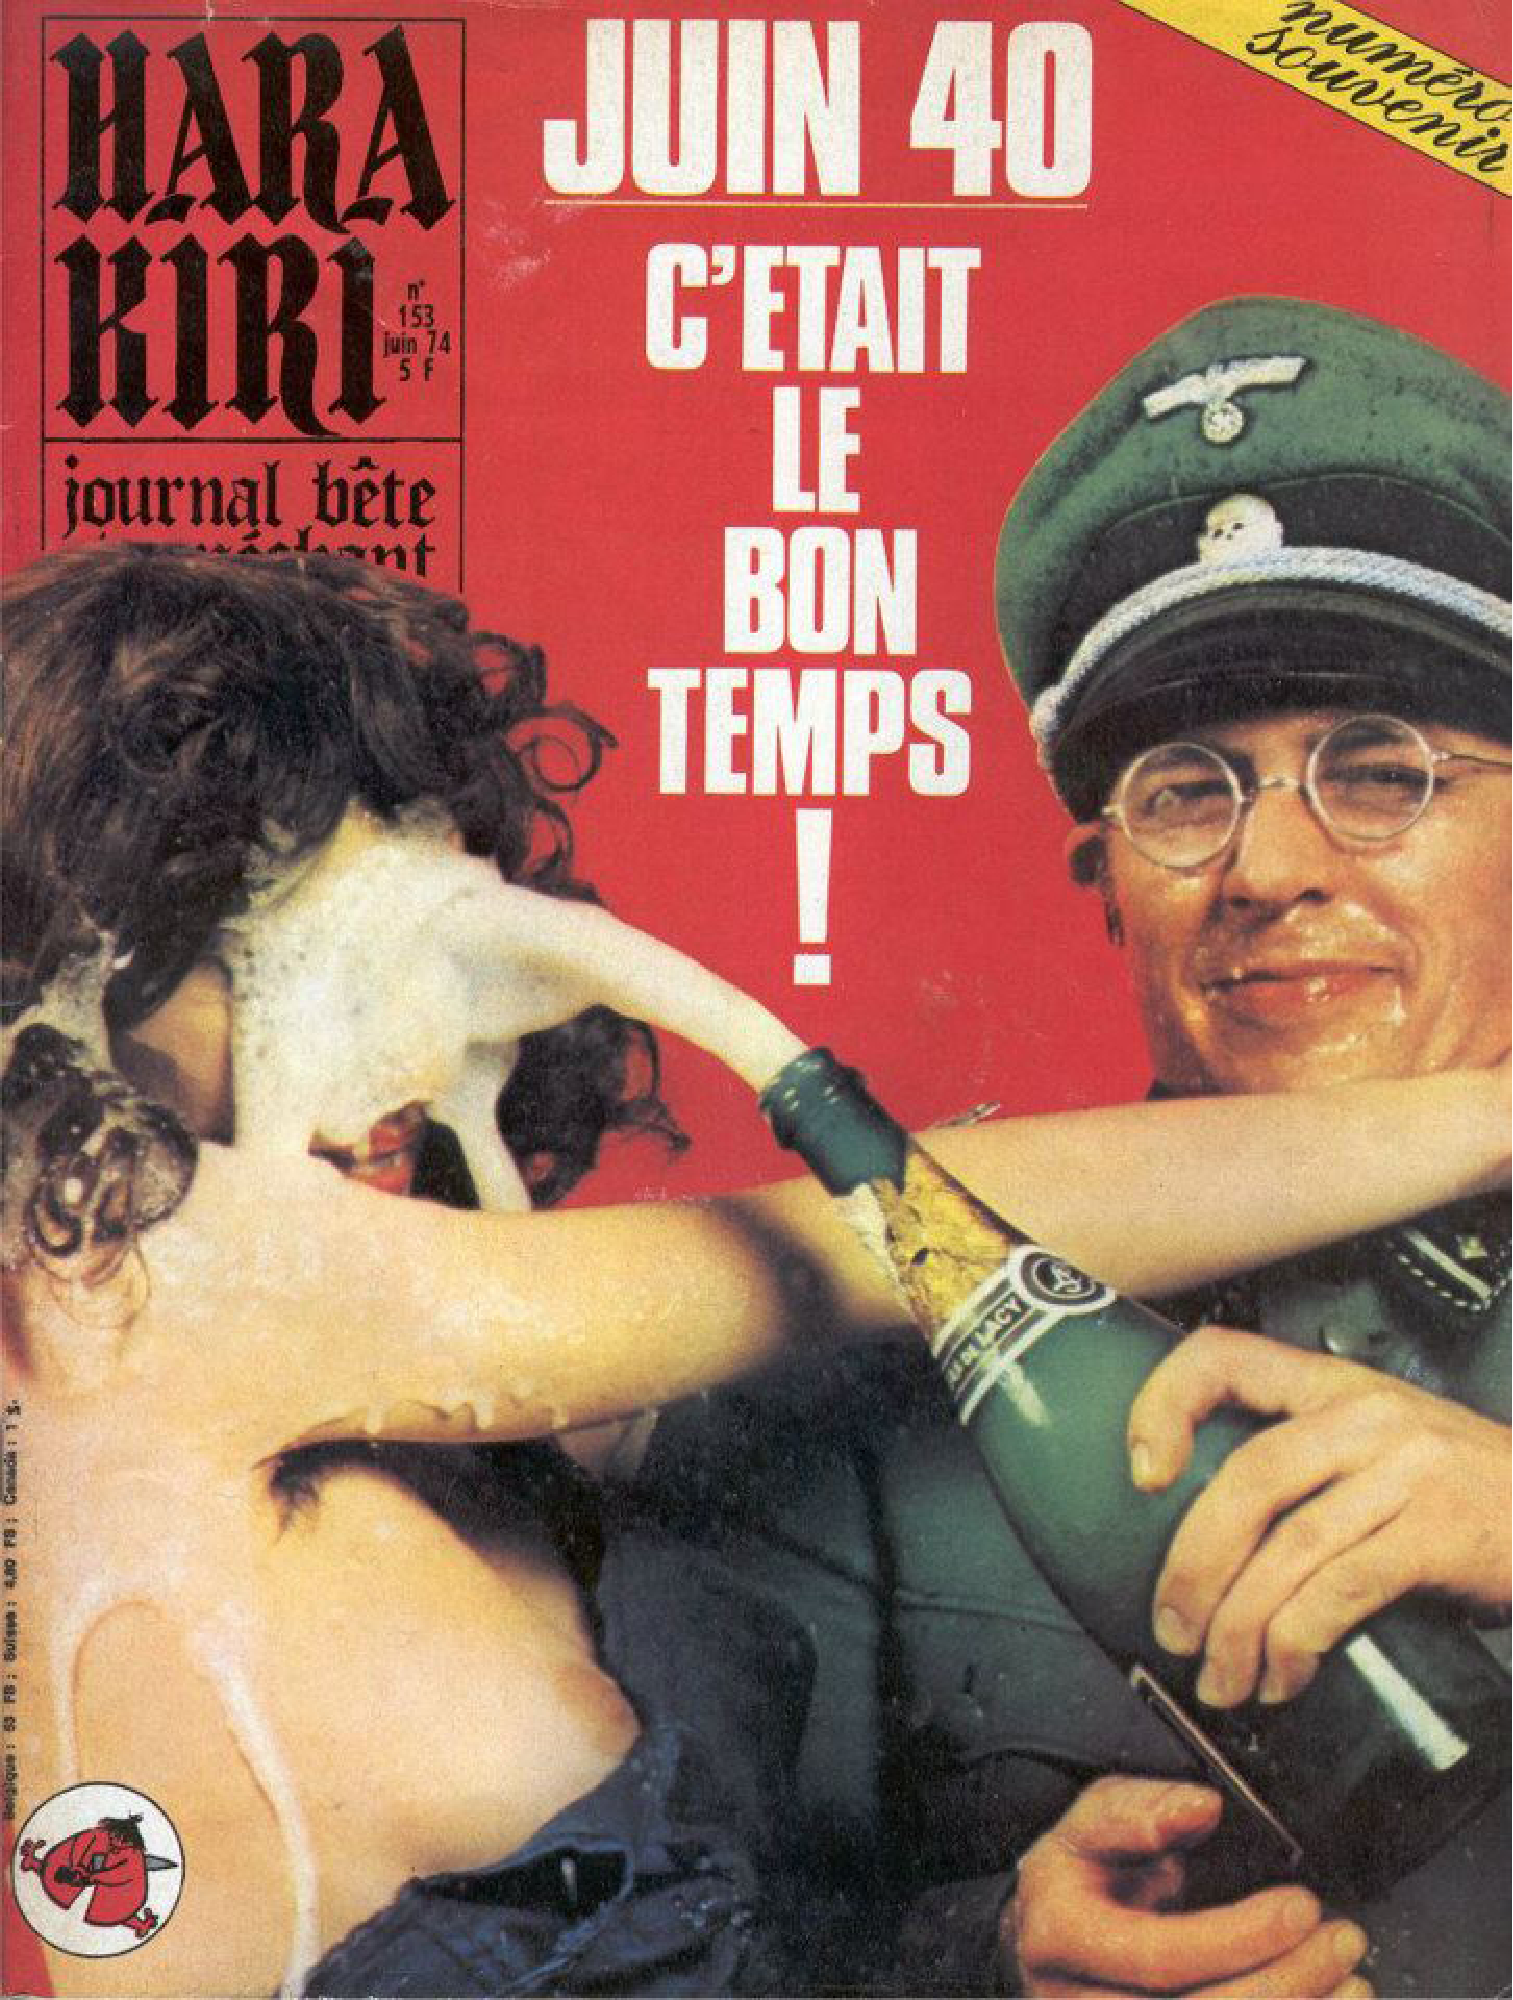
\includegraphics[width=8cm]{Fig02}
\caption{On parle souvent d'Europe, c'est un mot auquel, en France, on n'est pas encore tr{\`{e}}s habitu{\'{e}}. (...) Pour moi, Fran{\c{c}}ais, je voudrais que demain nous puissions aimer une Europe dans laquelle la France aura une place qui sera digne d'elle.}
\label{Fig2}
\end{center}
\end{figure}

Rentrons !\fg~Je rentre avec lui. Voil{\`{a}}. \og Cette terrasse, qu'il commence, c'est pour les oeufs {\`{a}} la coque ! Viens par ici !\fg~Alors, on remarque encore qu'il n'y avait personne dans les rues, {\`{a}} cause de la chaleur ; pas de voitures, rien. Quand il fait tr{\`{e}}s froid, non plus, il n'y a personne dans les rues ; c'est lui, m{\^{e}}me que je m'en souviens, qui m'avait dit {\`{a}} ce propos : \og Les gens de Paris ont l'air toujours d'{\`{e}}tre occup{\'{e}}s, mais en fait, ils se prom{\`{e}}nent du matin au soir ; la preuve, c'est que lorsqu'il ne fait pas bon {\`{a}} se promener, trop froid ou trop chaud, on ne les voit plus ; ils sont tous dedans {\`{a}} prendre des caf{\'{e}}s cr{\`{e}}me et des bocks~\cite{Discipline}. C'est ainsi ! Si{\`{e}}cle de vitesse ! qu'ils disent. O{\`{u}} {\c{c}}a ? Grands changements ! qu'ils racontent. Comment {\c{c}}a ? Rien n'est chang{\'{e}} en v{\'{e}}rit{\'{e}}. Ils continuent {\`{a}} s'admirer et c'est tout. Et {\c{c}}a n'est pas nouveau non plus. Des mots, et encore pas beaucoup, m{\^{e}}me parmi les mots, qui sont chang{\'{e}}s ! Deux ou trois par-ci, par-l{\`{a}}, des petits...\fg~Bien fiers alors d'avoir fait sonner ces v{\'{e}}rit{\'{e}}s utiles, on est demeur{\'{e}}s l{\`{a}} assis, ravis, {\`{a}} regarder les dames du caf{\'{e}}.
\begin{center}
\emph{ Dans un mois, dans un an, comment souffrirons-nous,\\. Seigneur, que tant de mers me s{\'{e}}parent de vous ?\\Que le jour recommence et que le jour finisse\\
Sans que jamais Titus puisse voir B{\'{e}}r{\'{e}}nice,\\
Sans que de tout le jour je puisse voir Titus ?}
\end{center}

Apr{\`{e}}s, la conversation est revenue sur le Pr{\'{e}}sident Poincar{\'{e}} qui s'en allait inaugurer, justement ce matin-l{\`{a}}, une exposition de petits chiens ; et puis, de fil en aiguille, sur Le Temps o{\`{u}} c'{\'{e}}tait {\'{e}}crit.

\begin{figure}[!htb]
\begin{center}

\includegraphics[width=8cm]{Fig03}
\caption{Le probl{\'{e}}me du gouvernement d{\'{e}}passe donc en ampleur le cadre d'un simple remaniement minist{\'{e}}riel. Il r{\'{e}}clame, avant tout, le maintien rigide de certains principes.}
\label{Fig3}
\end{center}
\end{figure}

Tiens, voil{\`{a}} un ma{\^{i}}tre journal, Le Temps !\fg~qu'il me taquine Arthur Ganate, {\`{a}} ce propos. \og Y en a pas deux comme lui pour d{\'{e}}fendre la race fran{\c{c}}aise ! - Elle en a bien besoin la race fran{\c{c}}aise, vu qu'elle n'existe pas !\fg~que j'ai r{\'{e}}pondu moi pour montrer que j'{\'{e}}tais document{\'{e}}, et du tac au tac.

Credo in unum Deum,

Patrem omnipotentem,

factorem c{\ae}li et terr{\ae},

visibilium omnium et invisibilium.

Et in unum Dominum Jesum Christum

Filium Dei unigenitum.

Et ex Patre natum ante omnia s{\ae}cula.

Deum de Deo, lumen de lumine, Deum verum de Deo vero.

%Genitum, non factum, consubstantialem Patri : per quem omnia facta sunt.


%Qui propter nos homines, et propter nostram salutem decendit de c{\ae}lis.


%Et incarnatus est de Spiritu sancto ex Maria Virgine :

%Et homo factus est.

%Crucifixus etiam pro nobis : sub Pontio Pilato passus, et sepultus est.

%Et resurrexit tertia die, secundum Scripturas.


%Et ascendit in c{\ae}lum : sedet ad dexteram Patris.

%Et iterum venturus est cum gloria, judicare vivos et mortuos : cujus regni non erit finis.

%Et in Spiritum sanctum, Dominum, et vivificantem : qui ex Patre Filioque procedit.

%Qui cum Patre et Filio simul adoratur, et conglorificatur : qui locutus est per Prophetas.

%Et unam, sanctam, catholicam, et apostolicam Ecclesiam.

Confiteor unum baptisma in remissionem peccatorum.

Et expecto resurrectionem mortuorum.

Et vitam venturi s{\ae}culi.

\section{Hiver 2017 : Laude}

Ce n'est pas moi qui vous bernerai par des paroles trompeuses~\cite{Foucault}. Je hais les mensonges qui vous ont fait tant de mal. La terre, elle, ne ment pas.

\begin{figure}[!htb]
\begin{center}
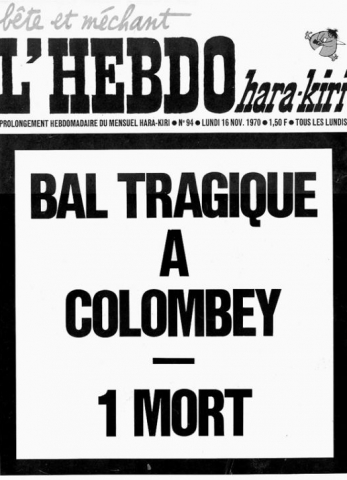
\includegraphics[width=8cm]{Fig04}
\caption{Va, va, c'est une affaire entre le Ciel et moi, et nous la d{\'{e}}m{\'{e}}lerons bien ensemble, sans que tu t'en mettes en peine.}
\label{Fig4}
\end{center}
\end{figure}

Elle demeure votre recours. Elle est la patrie elle-m{\^{e}}me. Un champ qui tombe en friche, c'est une portion de France qui meurt. Une jach{\`{e}}re {\`{a}} nouveau emblav{\'{e}}e, c'est une portion de la France qui rena{\^{i}}t.
	
\section{Printemps 2017 : Prime}
\begin{flushright}
\emph{\textbf{\small{Faut-il br{\`{u}}ler Sade ?}}}
\end{flushright}

Je vais vous r{\'{e}}pondre tout de suite. Je ne vais pas mal mais rassurez-vous un jour je ne manquerai pas de mourir.
	
\section{{\'{e}}t{\'{e}} 2017 : Tierce}

De temps en temps, on me dit, ou on me fait dire, Ben oui ! vous {\^{e}}tes l{\`{a}} - et c'est fort gentil {\`{a}} mon {\'{e}}gard - mais apr{\'{e}}s vous ce sera la pagaille ! Alors, quelques-uns sugg{\`{e}}rent que l'on institue la pagaille tout de suite, de mani{\`{e}}re {\`{a}} assurer ma succession. Eh bien ! je demande {\`{a}} r{\'{e}}fl{\'{e}}chir\ldots
	
\section{Automne 2017 : Sexte}

Bien entendu, on peut sauter sur sa chaise comme un cabri en disant l'Europe ! l'Europe ! l'Europe !\ldots mais cela n'aboutit {\`{a}} rien et cela ne signifie rien.
	
\section{Toussaint 2017 : None}

Il y a, pour ce qui est de la France, ce qui se passe dans une maison : la ma{\^{i}}tresse de maison, la m{\'{e}}nag{\`{e}}re veut avoir un aspirateur, elle veut avoir un frigidaire, elle veut avoir une machine {\`{a}} laver et m{\^{e}}me, si c'est possible, une auto : cela, c'est le mouvement.
	
\begin{figure}[!htb]
\begin{center}
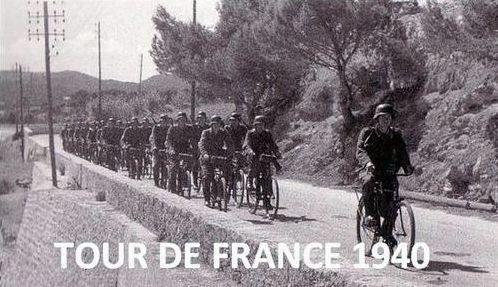
\includegraphics[width=14cm]{Fig05}
\caption{Ce n'est pas moi qui vous bernerai par des paroles trompeuses. Je hais les mensonges qui vous ont fait tant de mal. La terre, elle, ne ment pas. Elle demeure votre recours. Elle est la patrie elle-m{\'{e}}me. Un champ qui tombe en friche, c'est une portion de France qui meurt. Une jach{\'{e}}re {\`{a}} nouveau emblav{\'{e}}e, c'est une portion de la France qui rena{\^{i}}t.}
\label{Fig5}
\end{center}
\end{figure}

Et en m{\^{e}}me temps elle ne veut pas que son mari aille bambocher de toute part, que les gar{\c{c}}ons mettent les pieds sur la table et que les filles ne rentrent pas la nuit : {\c{c}}a, c'est l'ordre. La m{\'{e}}nag{\'{e}}re veut le progr{\'{e}}s mais elle ne veut pas la pagaille, eh bien ! c'est vrai aussi pour la France. Il faut le progr{\'{e}}s, il ne faut pas la pagaille\ldots
	
		
\section{D{\'{e}}cembre 2017 : V{\^{e}}pres}

Le pr{\'{e}}sident Lebrun prit cong{\'{e}}. Je lui serrai la main avec compassion et cordialit{\'{e}}. Au fond, comme chef de l'Etat, deux choses lui avaient manqu{\'{e}} : qu'il f{\^{u}}t un chef ; qu'il y e{\^{u}}t un {\'{e}}tat.
\newpage
\section{Conclusion}
\begin{flushright}
\emph{\textbf{\small{Arma Virumque Cano}}}
\end{flushright}
  La magnificence et la galanterie n'ont jamais paru en France avec tant d'{\'{e}}clat que dans les derni{\`{e}}res ann{\'{e}}es du r{\`{e}}gne de Henri second. Ce prince {\'{e}}tait galant, bien fait et amoureux ; quoique sa passion pour Diane de Poitiers, duchesse de Valentinois, e{\^{u}}t commenc{\'{e}} il y avait plus de vingt ans, elle n'en {\'{e}}tait pas moins violente, et il n'en donnait pas des t{\'{e}}moignages moins {\'{e}}clatants~\cite{Sade}.

Comme il r{\'{e}}ussissait admirablement dans tous les exercices du corps, il en faisait une de ses plus grandes occupations. C'{\'{e}}taient tous les jours des parties de chasse et de paume, des ballets, des courses de bagues, ou de semblables divertissements ; les couleurs et les chiffres de madame de Valentinois paraissaient partout, et elle paraissait elle-m{\^{e}}me avec tous les ajustements que pouvait avoir mademoiselle de La Marck, sa petite-fille, qui {\'{e}}tait alors {\`{a}} marier.

%\nonfrenchspacing

\begin{thebibliography}{99}
  
\bibitem{Noyau}Le noyau dirigeant de notre cause, c'est le parti communiste chinois.
 
 \bibitem{Fondement}Le fondement th{\'{e}}orique sur lequel se guide notre pens{\'{e}}e, c'est le marxisme-l{\'{e}}ninisme.
  
\bibitem{Revolution}Pour faire la r{\'{e}}volution, il faut qu'il y ait un parti r{\'{e}}volutionnaire.

\bibitem{Saminadayar}L. Saminadayar, \og \emph{Chroniques interdites}\fg, L. M. eds, (2018).
  
\bibitem{Parti}Sans un parti r{\'{e}}volutionnaire, sans un parti fond{\'{e}} sur la th{\'{e}}orie r{\'{e}}volutionnaire marxiste-l{\'{e}}niniste et le style r{\'{e}}volutionnaire marxiste-l{\'{e}}niniste, il est impossible de conduire la classe ouvri{\`{e}}re et les grandes masses populaires {\`{a}} la victoire dans leur lutte contre l'imp{\'{e}}rialisme et ses valets.
  
\bibitem{Efforts}Sans les efforts du Parti communiste chinois, sans les communistes chinois, ces piliers du peuple, il sera impossible {\`{a}} la Chine de conqu{\'{e}}rir son ind{\'{e}}pendance et d'obtenir sa lib{\'{e}}ration, il lui sera impossible {\'{e}}galement de r{\'{e}}aliser son industrialisation et de moderniser son agriculture.
  
\bibitem{Communiste}Le Parti communiste chinois constitue le noyau dirigeant du peuple chinois tout entier. Sans un tel noyau, la cause du socialisme ne saurait triompher.
  
\bibitem{Discipline}Un parti disciplin{\'{e}}, arm{\'{e}} de la th{\'{e}}orie marxiste-l{\'{e}}niniste, pratiquant l'autocritique et li{\'{e}} aux masses populaires ; une arm{\'{e}}e dirig{\'{e}}e par un tel parti ; un front uni de toutes les classes r{\'{e}}volutionnaires et de tous les groupements r{\'{e}}volutionnaires plac{\'{e}}s sous la direction d'un tel parti ; voil{\`{a}} les trois armes principales avec lesquelles nous avons vaincu l'ennemi.

\bibitem{Foucault}M. Foucault, \og \emph{Surveiller et punir}\fg, {\'{e}}ditions PCM (Plus Chiant tu Meurs), (1975).

\bibitem{Celine}L. F. Destouches dit C{\'{e}}line, \og \emph{Bagatelles pour un massacre}\fg, unpublished, (1937).

\bibitem{Sade}D. A. F. Sade dit Marquis de Sade, \og \emph{Les Cent Vingt Journ{\'{e}}es de Sodome}\fg, {\'{e}}ditions de la Pl{\'{e}}{\"{i}}ade, (1785, {\oe}uvre posthume).

 \end{thebibliography}

\end{document}